\documentclass[10pt,journal]{IEEEtran}

\usepackage[scale=0.8]{geometry}
\usepackage{graphicx}

% This centers the captions
\makeatletter
\long\def\@makecaption#1#2{\ifx\@captype\@IEEEtablestring
\footnotesize\begin{center}{\normalfont\footnotesize #1}
{\normalfont\footnotesize\scshape #2}\end{center}
\@IEEEtablecaptionsepspace
\else
\@IEEEfigurecaptionsepspace
\setbox\@tempboxa\hbox{\normalfont\footnotesize {#1.}~~ #2}
\ifdim \wd\@tempboxa >\hsize
\setbox\@tempboxa\hbox{\normalfont\footnotesize {#1.}~~ }
\parbox[t]{\hsize}{\normalfont\footnotesize \noindent\unhbox\@tempboxa#2}
\else
\hbox to\hsize{\normalfont\footnotesize\hfil\box\@tempboxa\hfil}\fi\fi}
\makeatother

\title{Design and implementation of the $sin$ function for an 8-bit MIPS processor}
\author{Dominik Laskowski, Payom Meshgin, Daniel Ranga, Ming Yang}

\begin{document}
\maketitle

\section{Introduction}
Hardware acceleration of transcendental functions is crucial for real-time systems
performing computationally intensive tasks like computer graphics and audio processing.
The x87 floating-point unit in the IA-32 architecture supports instructions like \texttt{fsin}
and \texttt{fsincos}. Likewise, graphics processing units and digital signal processors
provide dedicated logic for trigonometric operations.

Lookup tables based on ROMs and PLAs are the most common approach for implementing $sin$
in hardware. They are often coupled with approximation techniques like interpolation to
achieve adequate precision while reducing transistor count. An alternative method that
offers better precision at the expense of speed is the Taylor series expansion. Finally,
the CORDIC (for Coordinate Rotation Digital Computer) algorithm is desirable in embedded
systems without a multiplier, since it only requires adders, shifters and lookup tables.
In this report, we investigate the design and implementation of a $sin$ functional block for
an 8-bit MIPS processor, using the first two aforementioned approaches.

In practice, $sin$ blocks usually operate on 32-bit IEEE 754 floating-point numbers. However,
since the MIPS core has 8-bit registers and integer operations only, we opted for a custom encoding
scheme based on binary scaling. The assumed domain and image is $[0, \frac{\pi}{2}]$ and $[0, 1]$,
respectively. These ranges are discretized to an integer between $0$ and $255$.

\section{Lookup Table Implementation}

\begin{figure}[h]
\centering
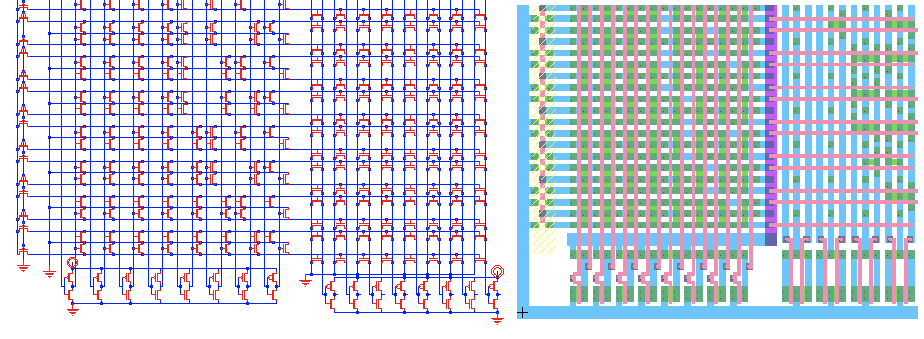
\includegraphics[width=3in]{lut.png}
\caption{Schematic and layout of the lookup table}
\label{lut}
\end{figure}

\begin{figure}[h]
\centering
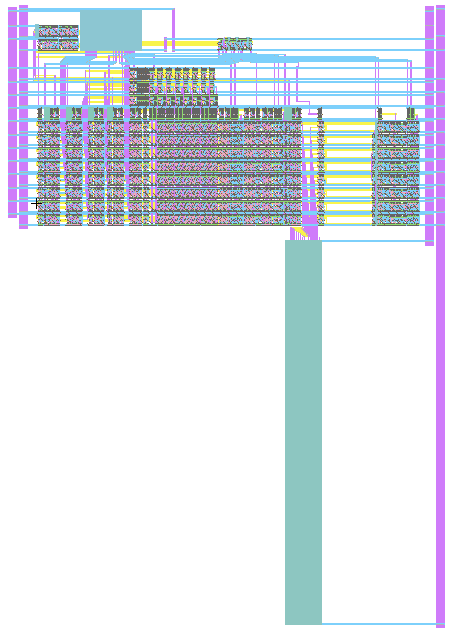
\includegraphics[width=3in]{mips_lut.png}
\caption{Layout of MIPS core with lookup table}
\label{mips_lut}
\end{figure}

\section{Taylor Series Implementation}

\section{MIPS Integration}

\section{Validation}

\section{Results}

\section{Conclusion}

\end{document}
